%!TEX program = lualatex
%!TEX encoding = UTF-8 unicode
%use lualatex compiler
\documentclass{article}
\usepackage[utf8]{inputenc}
\usepackage{csquotes}
\usepackage[english]{babel}
\usepackage{dblfloatfix}
\usepackage[sort,nocompress]{cite}
\usepackage{hyperref}
\usepackage[shortlabels]{enumitem}
\usepackage[nottoc,notlot,notlof]{tocbibind}
\usepackage{url}
\usepackage{mathtools}
\usepackage{pgfplots}
\DeclarePairedDelimiter{\ceil}{\lceil}{\rceil}
\hypersetup{
    colorlinks,
    citecolor=black,
    filecolor=black,
    linkcolor=black,
    urlcolor=black
}

\title{My Gambling Experience and Lessons}
\author{Atipat Lorwongam}
\date{5 November 2020}

\usepackage{listings}
\usepackage{color}
\definecolor{white}{rgb}{1,1,1}
\definecolor{dkgreen}{rgb}{0,0.6,0}
\definecolor{gray}{rgb}{0.5,0.5,0.5}
\definecolor{mauve}{rgb}{0.58,0,0.82}
\definecolor{cream}{rgb}{1, 0.992, 0.816}
\definecolor{lightyellow}{rgb}{1, 1, 0.875}

\setlength{\parindent}{4em}

\lstset{frame=tb,
  language=C,
  aboveskip=3mm,
  belowskip=3mm,
  showstringspaces=true,
  columns=flexible,
  basicstyle={\small\ttfamily},
  numbers=none,
  numberstyle=\tiny\color{gray},
  keywordstyle=\color{blue},
  commentstyle=\color{dkgreen},
  stringstyle=\color{mauve},
  breaklines=true,
  breakatwhitespace=true,
  tabsize=4
}


\begin{document}
\pagecolor{lightyellow}
\maketitle
\tableofcontents
\newpage

\clearpage
\section{Preface}
\paragraph{ }
I have been in gambling since 2012 after I was invited to join a management trip to a casino ship in Hong Kong.  That was my first time in a casino.  With the mind of an engineer,  I tried to make sense of it out of mathematics and tried to configure how to win casino money ever since.\\
	
The purpose of this paper is to prove and analyze the game of gambling and show why the casino is not beatable mathematically.  For that, some basic algebra and statistics are needed for the readers.\\
	
This paper is not to promote gambling or otherwise, but to give a perspective from my own experience being in this area for some time.  I will try to make it readable the best I can.  Since my first language is not English, then writing an academic paper in English is somewhat a challenge to me.  But I will try it anyway.  \\

	All my trips to the casinos were never much for the money but to test out, find out a theory that I assumed.  After tested with games and seen some results, at that moment I would want to try in real places.  Lots of tries and errors taken, and yes, I had fun and somewhat addicted, but I was sure, I was in control of my own emotions, and actions, or at least I have full intention to do so.\\
	
	I was born in a family that gambling is evil, which is not far from the truth, I think since there are lots who lost their families, assets, or their lives to the devil.  My family prepared me well, that they pointed out the dark sides of gambling.  So, to touch in this area, I had to have patience and be disciplined to make sure I will not be a victim of the devil myself.  I gathered lots of information and learned from all information I can get online, which is plenty. \\
	
	My interest in gambling went from \emph{Want to win} \rightarrow \emph{I can find a way to win} \rightarrow \emph{want to create my Strategy} \rightarrow \emph{Learn the math behind it} \rightarrow \emph{Find the strategy that mathematically wins} \rightarrow \emph{Tested out with math and games} \rightarrow \emph{Review and improve} \rightarrow \emph{Move on to various games} \rightarrow \emph{Final Summary}\\
	
	In the end, I had to move on to other games because I found that almost all the  games in the casino are unbeatable!  Every game in the casino is well thought and calculated.  That is guaranteed to win casino money. and that is why the casino business will never go bankrupt unless there are not well managed. \\
	
	I will try to tell you my story, and some naive though I had.  Therefore, you might find that math, in the beginning, is tempting and naive!  But please, do not run to a casino just yet.  Finish the paper then you will learn what I am trying to tell you.\\

\clearpage
\section{My First Gambling Strategy}
\paragraph{ }
The first game I started, was the game of Baccarat.  After a while, I found that even close 50-50 game things are not as expected.  I first thought of using a strategy called "Martingale" progressive betting system which I thought that there is no way a game with a possibility nearly close to 50-50 would have a forever long streak of winnings or losings.\\

At first, I won many trips in a row, using Martingale's, this made me think that "there I found the strategy that can earn me the money" without knowing that was too easy and was just a tip of an ice burg.  Which not long later I found that there was a streak of lost trips and dried out my bankroll.\\

It made me wonder what happened.  I started to think more than just "Martingale strategy" and learn more about other "Progressive betting strategies" and tried to get to the math behind it!\\
\subsection{Martingale Strategy}
\paragraph{ }
	It is based on the idea that if you keep betting in a 50-50 game you will eventually win, in other words, you will never lose forever.  So, based on that assumption each Martingale's strategy wins a minimal amount win but a large bankroll is required.\\
	
To calculate Martingales, we must assume that everyone has a limited amount of bankroll.  It is no doubt that if one has an unlimited bankroll, he/she can double their bet forever to win such a small amount.  Then, if they had such a large amount of money (virtually unlimited amount), a small win will not satisfy them, and they have no reason to gamble in a casino.\\

Or even if the player has an unlimited amount of bankroll, he/she will be limited by the casino rules anyway  (Maximum bet).  That is, there will be $n$ time that he/she can double his/her bets, and $n\neq\infty$.\\

	Assume that $p_b$ is Baccarat probability, which we thought 1 outcome out of 2, that is $\frac{1}{2}$.  So, I thought the probability of we will lose 6 or 8 times in a row is slim. How slim? If we let $n$ be the number of times we keep losing in a row, and $p_{l_n}$ is the total probability of losing $n$ time in a row we get:\par
\begin{center}
$p_{l_n}=p_b^n$
$$p_{l_n}=(\frac{1}{2})^n$$\\(2.1)
\end{center}
  From this we have:\\
\begin{center}
$p_{l_6}=(\frac{1}{2})^6=\frac{1}{64}=0.015625\approx1.56\%$\\
$p_{l_7}=(\frac{1}{2})^7=\frac{1}{64}=0.0078125\approx0.56\%$\\
$p_{l_8}=(\frac{1}{2})^8=\frac{1}{256}=0.00390625\approx0.4\%$\\ 
\end{center}
That is, there are only about \approx1.56\%, \approx0.56\%, \approx0.4\% to lose 6, 7, and 8 times in a roll accordingly.  \\

We know that all probability should sum up as 1. So, we have win probability $p_{w_n}$ would be:\par
\begin{center}
	$$p_{w_n}=1-\frac{1}{2}^n$$\\(2.2)\\
\end{center}
  From this we have:\\
\begin{center}
	$p_{w_6}=1-\frac{1}{2}^6=1-\frac{1}{64}=0.984375\approx98.43\%$\\
	$p_{w_7}=1-\frac{1}{2}^7=1-\frac{1}{64}=0.9921875\approx99.22\%$\\
	$p_{w_8}=1-\frac{1}{2}^8=1-\frac{1}{256}=0.99609375\approx99.61\%$\\
\end{center}

From above the math, we have that chances of winning for 6, 7 and 8 games in a row are \approx98.43\%, \approx99.22\%, \approx99.61\% accordingly.  \\

from the possibility above that surely fooled me and lots of gamblers.  That they would think, there will be just only 0.4\% probability they could lose their 8 times in a row.  They would think, for the bankroll needed for 8 times lost they would almost be guaranteed to win.\\

The actual Martingale's Progressive betting strategy, says that you \emph{start at a minimum bet, for the next bet should double your bet every time you lose, and for each win, you should start at the minimum amount again}, and you will also win a minimum amount for each win.  It is a proven strategy shown below:\\

let $b_n$ is bet amount at game $n$, and $b_{total_n}$ is total bet amount at game $n$ and $w_n$ are the amounts won at game $n$. \\

For each game win summary is a sum of current game $n$ won minus sum of total bet to previous game $n-1$, let $total_n$ is a win summary at game $n$, we have that:\par
\begin{center}
$$total_n = w_n - b_{total_{n-1}}$$\\(2.3)\\
\end{center}

Baccarat by approximate pay 1:1, so we have bet amount equal won amount.  We double each bet at each game if $a_{min}$ refer to minimal bet amount, we have:\par
\begin{center}
 $w_n = b_n = a_{min} * 2^{(n-1)}$\\
\end{center}
If we let $a_{min}=1$ for $1$ unit, we have:
\begin{center}
 $$w_n = b_n = 2^{(n-1)}$$\\(2.4)\\
\end{center}

Total loss at game $n$ that means we lost every game to the game $n-1$, we have:\par
\begin{center}
$b_{total_{n-1}} = a_{min} * (b_1+b_2+b_3+...b_{n-1})$\\
$b_{total_{n-1}} = a_{min} * \sum^{n-1}_{i=1}b_i$\\
$b_{total_{n-1}} = a_{min} * (2^{(n-1)}-1)$\\
\end{center}
Again, if we let $a_{min}=1$ for $1$ unit, we have:
\begin{center}
$$b_{total_{n-1}} = 2^{(n-1)}-1$$\\(2.5)\\
\end{center}
From (2.3), (2.4), (2.5) we have:\\

\begin{center}
	$total_n = 2^{(n-1)}-(2^{(n-1)}-1)$\\
	$total_n = 2^{(n-1)}-2^{(n-1)}+1$\\
	$$total_n = 1$$\\(2.6)\\
\end{center}
QED\\

We have proven that for every win in $n$ games lost in a row, you will win 1 unit of minimum bet amount $a_{min}$. And you will need a large bankroll $b_{total_n}$ shown below:\\
\begin{center}
$$b_{total_n}=\sum^n_{i=1}b_i$$\\
$$b_{total_n}={2^n}-1$$\\(2.7)
\end{center}
\begin{center}
\begin{tikzpicture}
  \begin{axis}[ 
  	xmin=-1,
  	xmax=10,
    xlabel=$n$,
    ylabel={$f(n) ={2^n}-1$}
  ] 
    \addplot [domain=-1:10]{2^x-1}; 
  \end{axis}
\end{tikzpicture}
\end{center}

From the graph above we can see that the amount of bankroll needed is rising exponentially.  

\subsubsection{Selling a Dream}
from (2.7) we found that to be able to lose 8 games in a row, we will need a total bankroll of:\par
\begin{center}
$b_{total_n}={2^n}-1$\\
$b_{total_8}={2^8}-1$\\
$b_{total_8}=255$\\
\end{center}

255 unit of minimal bet amount $a_{min}$.  That is, if we are at a 100\$ minimum bet table, we will need a bankroll of $a_{min} * 255 = 25,500\$$ to be able to implement this strategy with $n=8$ game.  We have a win probability of \approx99.61\%.  This sounds good. Because it is almost a guarantee every win. that is less than half a percent chance that we will lose. \\

sounds good??\\

And if we play 100 games 1 time it almost guarantees that we will win 99 times, because 0.4\% means that we will only lose 4 games in 1,000 games and we are almost guaranteed to win $\approx100*99.61\approx9961\$$ for 100\$ games.  sounds good right?
\subsubsection{the Truth}

After 6-8 times going to the casino, I found that I sometimes win, sometimes lose, so I summed it all up.  I found that I almost win a bit but if I include the cost of the hotel and transportation, I lost lots of money in the process to the casino.  But hey! I had fun!\\

After that, I started to go big, invited friends to come to even bigger casinos, sometimes I lost big at the first play of going big bet!  I was getting more stressed, then after $2$ or $3$ trips, I got them back.  But never long, it finally got to the point that I am sure that I can never get them back with this strategy.\\

All these times, I was trying to make sense of what was happening. I was mentally ill that I blamed myself for the casinos' benefits. I blamed myself for what I did not do right, what should I have done.  But in the end, it was just about what should have I done to win money in the long run.  I suspected, how many rounds $n$ to count before I should let go of the losses (in terms of investment called "cut loss") and restart the series to the minimum bet.  So, I researched harder, and during this period I learned lots of concepts and strategies to try other progressive systems other than Martingales.  I will describe later in \emph{Other Progressive Betting Systems}.\\

One thing I found during that time, if the game was true 50-50, in other words, the chance to win and lose is equal $\frac{1}{2}=0.5=50\%$, then the sum of overall wins and losses should equal zero! \\

Let $total$ is a total win/lose summary, and suppose $w_{total}$, $l_{total}$ is a total win that we won/lost in all the sessions, accordingly, which $w_{total}$ can be calculated by the \textbf{amount win} times \textbf{chance to win}, and $l_{total}$ can be calculated by The \textbf{amount will be lost} (In this case will be the sum of the whole series of bet amount shown in (2.7)) times \textbf{chance to lose}.  If we sum them up, we will get a total win or lose for this strategy.\\

Since return rate $r$ will be applied for every time we win. so, we use $r^n$ in the equation, but the rate of loss will always equal $1$ so, we will just leave it out.  We have:\par
\begin{center}
$total = w_{total}-l_{total}$\\
$total = r^n*p_{w_n} - b_{total_n}*p_l^n$\\
$total = r^n(1-p_l^n)-(2^n-1)*p_l^n$\\
$total = r^n-r^np_l^n-2^np_l^n+p_l^n$\\
$total = r^n-p_l^n(2^n+r^n-1)$\\
(2.8)
\end{center}
let us plug all the values and assume that $r=1$ we have:\par
\begin{center}
$total = 1-\frac{1}{2}^n(2^n+1-1)$\\
$total = 1-1$\\
$total=0$\\
\end{center}
QED\\

From the above QED, we proved that in the end, the sum of wins and losses will equal 0, in other words, the winning and losing from this strategy are just the same amount.  In the long run, we will very much not gaining nor losing money, but ...\\

Unfortunately, in the real-world scenario, we will lose more money because of two factors.
\begin{itemize}
\item One is that we pay for transportation, meals, and accommodations for this non-sense trip (or just for fun).
\item Two, to be precise, I learned that Baccarat is not a 50-50 game but more of a \textbf{0.458597~0.446247} game.  To understand this, I must explain how Baccarat is played.
\end{itemize}

\clearpage
\section{How Baccarat is Played}
\paragraph{}
Baccarat is played by players against the house (Casino).  Players will each choose a choice either \emph{Blue} or \emph{Red}, generally Blue stands for \emph{PLAYER} and Red for \emph{BANKER}.  The dealer will then start dealing with 2 initial cards for each Player and Banker.  \par
\begin{center}
\emph{** note **}\\
\textit{Player Box does not refer to players' hands, and Banker Box does not refer to the casinos. They are just two boxes for players to make a choice.}\\
\end{center}

\paragraph{}
After the cards are dealt, Player Box will be turned over first, to sum up, the point.  The value of the cards will be summed up with 10s and face cards are counted as 10.  After all the point is summed up only the last digit will be taken to account.  For example, 13 is counted as 3, 25 is counted as 5, 21 is counted as 1, and 20 is counted as 0 and this is the worst score in Baccarat.\\

The Player hand will then have one more chance to improve its hand by taking one more additional card which is standardized Baccarat around the world.  The player hand will deal with one additional card if it has a score of less than 6.  After summing up with the \emph{additional card}, that will be the final score for the Player Box.  \\

Then the dealer will turn over Banker Box and check to score.  After summing up the score in the same way, the Banker Box will take a card or stand will depend on two factors.

\begin{itemize}
\item \emph{Player's additional card} \textbf{NOT the score}
\item Banker's total score
\end{itemize}

The rules are shown in table 1.  For each Banker's score on the left, the dealer will act corresponding to the Player's additional card listed horizontally in the column.\\

\begin{table}[htb]  
%[htb] table optios to put in place with paragraph other wise it be at the top of a page
\centering
\begin{tabular}{|c|c|c|c|c|c|c|c|c|c|c|}
\hline
Player Card & 0 & 1 & 2 & 3 & 4 & 5 & 6 & 7 & 8 & 9\\
\hline  
0 & d & d & d & d & d & d & d & d & d & d\\
1 & d & d & d & d & d & d & d & d & d & d\\
2 & d & d & d & d & d & d & d & d & d & d\\
3 & d & d & d & d & d & d & d & d & s & d\\
4 & s & s & d & d & d & d & d & d & s & s\\
5 & s & s & s & s & d & d & d & d & s & s\\
6 & s & s & s & s & s & s & d & d & s & s\\
7 & s & s & s & s & s & s & s & s & s & s\\
8 & s & s & s & s & s & s & s & s & s & s\\
9 & s & s & s & s & s & s & s & s & s & s\\
\hline

\end{tabular}
\caption{shows the \emph{BANKER} action table.  \emph{d}: draw, \emph{s}: stand}
\end{table}

After Banker Box draws one additional card or stands according to table 1, then we start to compare the final score.  If the Player Box score is higher than Banker Box, then the Player Box won and vice versa.  \\

This is a normal play, but there are some special notes and conditions to the game of Baccarat, which will be described below.\par

\begin{description}
	\item[natural hands] if Player or Banker box has eight or nine with 2 cards the game ends and the comparing score start right away.
	\item[tie] if the scores are tie all bets are a push.  and if you bet on tie the payout is 8 to 1, but trust me, do not ever think of betting on tie.
	\item[payout] if Banker is your choice and if Banker won, the casino would pay only 95\% of your bet, but you will be paid 100\% if you are betting the Player Box.
\end{description}

According to the rule above, some websites calculated all combinations for all outcomes. One of the very well-known websites in the gambling industry is \url{https://www.wizardofodds.com} AKA \emph{Wizard of Odds}.\par

\begin{table}[htb]
\centering
\begin{tabular}{|c|c|c|c|c|}
\hline
Event & combinations & Probability & Payout & no-tie prob\\
\hline
Banker win & 2,292,252,566,437,888 & 0.458597423 & 0.95 & 0.50682483\\
Player win & 2,230,518,282,592,256 & 0.446246609 & 1 & 0.49317517\\
Tie & 475,627,426,473,216 & 0.095155968 & 8 & \\
\hline
\end{tabular}
\caption{shows Baccarat probability and payout for each outcome}
\end{table}

You might think "this is not bad" but, it is already worse than the 50/50 game we assumed earlier. why? Let us get to know the concept of \emph{Expected Value}.  

\clearpage
\section{Expected Value (EV)}

We already touched on a little bit of the Expected Value concept before, you might not realize.  It was when we were trying to describe a 50-50 game with Martingale's betting strategy outcome and proven it to be equal in the total result.\\

Imagine that you have won lots of games and accumulate lots of winnings and suddenly just one lost you lose all the money you had accumulated and/or even more!  Expected Value (EV) is a concept that is used to calculate any investment situation that has a chance and risk involved.\\
\\
3 ways Expected Value outcomes could be. They are: \par
\begin{description}
\item[Positive EV] shows that investment with the calculated chance, risk, and reward is profitable.  The larger this number the better.  This means more profit for the investor.
\item[Negative EV] shows that investment with the calculated chance, risk, and reward is NOT profitable.  This is the opposite of a positive EV that is the larger the negative number is, the worse.  and we should not invest in this game or strategy.
\item[Zero EV] shows that investment with the calculated chance, risk, and reward is Fair.  That is in the long run, betting or investing in this project or strategy will get you nowhere.  
\end{description}

Let us get to the more important part, how do we calculate these expected values.  As we did, proved the total value of an assumed-50-50-game of Baccarat.  \\

Let us recap what we did.  we calculated the overall wins by the amount expected to win (from now on we will call it \emph{"Return"}) multiply by the chance of winning (from now on we will call it \emph{chance}).   Then, we calculated the overall losses by multiplying the total amount of losses (from now on we will call it \emph{"Loses"}) and chance to lose (From now on we will call it \emph{risk}).  Lastly, we summed them up.  And that exactly how we calculate the Expected Value.\\

Put it this way \textbf{Expected Value (EV)}, is a sum of the weighted average of all wins/losses possible outcomes.  That is, all cases with wins losses must be considered.  If we have $c_w$, $c_l$ for winning and losing cases of probabilities  $E_R, E_L$ we can calculate $E_V$ as:\par
\begin{center}
$$E_V=\sum_{i=1}^{c_w}E_{R_i}+\sum_{i=1}^{c_l}E_{L_i}$$\\(4.1)\\
\end{center}

In short, the Expected Value (EV) is a total value of Expected Returns (ER) and Expected Losses (EL).  from the explanation, we can have mathematically written as:\par
\begin{center}
$$E_V=E_R+E_L$$\\(4.2)\\
\end{center}
If we let $R$ for Return rate, $C$ for Chance, or possibilities of winning, $L$ for Lose rate, and $K$ for Risk or possibilities of losing, we can calculate Expected Return $E_R$ and Expected Lose $E_L$ as:\par
\begin{center}
$$E_R=R*C$$ \\ (4.3) \\
$$E_L=L*K$$ \\ (4.4) \\
\end{center}

From (4.2), (4.3), and (4.4) we can have an overall way of describing EV in mathematics as:\par
\begin{center}
$$E_V= R*C+L*R$$\\ 
(4.5)\\
\end{center}

From the Baccarat Probabilities in Table 2, we can calculate the real Expected Value of Baccarat using the (4.5) formula as:\\ \\
\emph{If we are betting on the Banker side: $E_{V_b}$}
\begin{center}
$E_{V_b}=R_b*C_b+L_b*K_b$\\ 
$E_{V_b}=0.95*0.50682483+(-1)*0.49317517$\\ 
$E_{V_b}=0.481483588-0.49317517$\\
$E_{V_b}=-0.011691582$\\
\end{center}
\emph{If we are betting on the Player side: $E_{V_p}$}
\begin{center}
$E_{V_p}=R_p*C_p+L_p*K_p$\\ 
$E_{V_p}=1*0.49317517+(-1)*0.50682483$\\ 
$E_{V_p}=0.49317517-0.50682483$\\
$E_{V_p}=-0.01364966$\\
\end{center}

Alright, let us calculate the tie bet for Baccarat mentioned, do not bother betting on it.  From Table 2, we have a probability of game-tying in Baccarat and payout. Let $E_{V_t}$  is expected value for tie and $p_t$ is the probabilities of Baccarat result in a tie, we have:\par
\begin{center}
$E_{V_t}=R_t * C_t + L_t * K_t$\\
$E_{V_t}=8 * 0.095155968 + (-1) * (1-C)$\\
$E_{V_t}=0.761247744 - 0.904844032$\\
$E_{V_t}=-0.143596288$\\
\end{center} 

From the above EVs betting on tie has a whopping -14.36\% while betting on Banker or Player Box will also guarantee you to lose, but at a slower rate about \approx0.01\approx1\% for any amount you bet or invest in either box. \\ 

We now know that the Expected Value on either side (Banker Box or Player Box) is negative.  Even ties, also result in an even larger negative expected value. In summary, no matter player is betting on Banker or Player side or even tie, in the end, players are guaranteed to lose.  \\

Finally, we can just summary that EV is the rate that they must pay per play.  For example, if the player is betting Player Box in baccarat of $E_{V_p}=-0.01364966$ this means on average the player will pay about \approx1.364966\% of his bet per play.\\

\subsection{Expected Value to martingale}

As we can see Expected Value on Banker and Player is different than what we assumed, it is not a 50-50 chance.  So, our assumption, in the beginning, cannot be used.  We must recalculate EV for Martingale's Strategy on Banker and Player separately.  Again, we will leave the minimum amount $a_{min}$ out to just calculate the rate of EV, by assuming that the $a_{min}=1$.\\

From Equation (2.1) we can say that the risk of the game will be $p_l^n$ if $p_l$ is a probability of losing the whole n number long series.  According to (2.2), the chance of winning would be $1-p_l^n$.  As we double the amount we bet for each game, same as before, so we have the same solution for the total loss and winning amount as before $b_{total_n}$, $w_n$ accordingly. This time let us do it in a more general way by putting a return rate $r$ in the equation, so that we can calculate EV for Martingale's Strategy on any game $E_{V_m}$ as below: \\

In Martingale's every win, win 1 unit of $a_{min}$ and risk the whole bankroll $b_{total_n}$ for it.  We can write the $E_{V_m}$ equation as below:\\ \\
As for every game-winning $r$ is repeated so, in this equation, we use $r^n$, and for every loss we lose 1 so the loss rate will be $1^n=1$ :\par 
\begin{center}
$E_{V_m}=r^n(1-p_l^n)-1^nb_{total_n}*p_l^n$\\
$E_{V_m}=r^n(1-p_l^n)-(2^n-1)*p_l^n$\\
$E_{V_m}=r^n-r^np_l^n-2^np_l^n+p_l^n$\\
$$E_{V_m}=r^n-p_l^n(2^n+r^n-1)$$\\
(4.6)\\
\end{center}

\subsubsection{True Martingales' EV on Player}
From Equation (4.6), while $p_l$ is the probability of the Banker, we can calculate the Expected value for player $E_{V_{m_p}}$ as below: \\

\begin{center}
$E_{V_{m_p}}=r^n-p_l^n(2^n+r^n-1)$\\
$E_{V_{m_p}}=1-0.50682483^n(2^n)$\\
\end{center}
\begin{center}
\begin{tikzpicture}
  \begin{axis}[ 
  	%axis x line=middle,
  	%axis y line=middle,
  	%axis equal,
    xlabel=$n$,
    xmin=-1,
    xmax=10,
    ymin=-0.5,
    ymax=0.5,
    ylabel={$E_{V_{m_p}}=1-0.50682483^n(2^n)$}
  ] 
    \addplot [domain=-1:10]{1-0.50682483^x*2^x}; 
  \end{axis}
\end{tikzpicture}
\end{center}
We can be precise by calculating (4.6) while $n=8$:\par
\begin{center}
$E_{V_{m_p}}=1-0.50682483^8(2^8)$\\
$E_{V_{m_p}}=1-0.004353746*256$\\
$E_{V_{m_p}}=-0.11455892$\\
\end{center}

That is, you will lose \approx11.456\% every time you bet using this strategy! I have calculated for $n=7$ and $n=6$ for you, the $E_{V_{m_{p_7}}}=-0.099550431$, $E_{V_{m_{p_6}}}=-0.084744043$.  This means that the larger $n$ is, the larger the rate of losses.  

\subsubsection{True Martingales' EV on Banker}
As we did on Player, from Equation (4.6), this time we can say that the risk of the game $p_l$ will be the probability of Player win. We can calculate $E_V$ for Martingale's strategy betting Banker Box $E_{V_{m_b}}$ as below: \\
\begin{center}
$E_{V_{m_b}}=r^n-p_l^n(2^n+r^n-1)$\\
$E_{V_{m_b}}=0.95^n-0.49317517^n*(2^n+0.95^n-1)$\\
\end{center} 
\begin{center}
\begin{tikzpicture}
  \begin{axis}[ 
  	%axis x line=middle,
  	%axis y line=middle,
  	%axis equal,
    xmin=-1,
    xmax=10,
    ymin=-0.5,
    ymax=0.5,
    xlabel=$n$,
    ylabel={$E_{V_{m_b}}=0.95^n-0.49317517^n*(2^n+0.95^n-1)$}
  ] 
  \addplot [domain=-1:10]{0.95^x-(0.49317517^x*(2^x+0.95^x-1))}; 
  \end{axis}
\end{tikzpicture}
\end{center}
To calculate $n=8$: we have:\par
\begin{center}
$E_{V_{m_b}}=0.95^8-0.49317517^8*(2^8+0.95^8-1)$\\
$E_{V_{m_b}}=0.663420431-0.003499529(256+0.663420431-1)$\\
$E_{V_{m_b}}=-0.231281179$\\
\end{center}

That is, you will lose \approx23.128\% every time you bet using this strategy! I have calculated for $n=7$ and $n=6$ for you, the $E_{V_{m_{b_7}}}=-0.207799285$, $E_{V_{m_{b_6}}}=-0.181942946$.  Hope this make sense to you \\

Therefore, unless there is no maximum bet limitation, in other words, $n\rightarrow\infty$ which will make our first assumption true.  Since that is not the case, in the real-world, $n$ is a limited integer.  So, this EV calculate is the truth, the larger $n$ is, the more money you will be losing.  \\

So, one thing I did and tried was, I did not just double bet but triple the bet and tried to reduce the number of $n$.  Hoping things would be better, but that is not the case.  I was not as smart as I thought I was, that was stupid!  Because of switching multiplier from 2 to even bigger number means a larger base of exponential That also making things worse!  (I will discuss this in \emph{Other Progressive Betting System})\\

\subsection{Learn Expected Value and Wake up}

As described previously that I was lucky that I did not lose much before I put my mind systematically thought this through.  I found that I was at least lucky enough that I did not lose big to these false strategies.  \\

I once took a friend to gamble in a big casino, we put our money together, we had a big bankroll, that I thought the "Martingale Variation" would benefit us with a large bankroll.  We had a night to play.  What happened was, only one bad luck, our bankroll was wiped out in just 2 hours of play.  So, we had only one choice, but to walk around in the hotel and the casino, no more playing for the whole trip.\\

So, guys, I encourage you to learn the concept of the \textbf{Expected Value} and wake up!\\

After that I put my mind into math, only trust in math.  I will calculate my EVs for my strategies and test them (in excel, in programs, in games) out before I go to a real casino.  Here is my secret, after that, I play less, I only play for fun, and I changed to the game that I likely coming out ahead of.  I can say that I had fun and never have to give them money ever since! (because it all intentionally planned out, and I only pay what I can afford to have fun)\\

\subsection{What is a House Edge?}
If you have been researching for some time, you might come across the word \emph{"House Edge"} or \emph{"House Advantage"} it is referred to the casinos' advantage in the game which can be calculated by the \textbf{casino's expected values} divided by \textbf{cost per play}. \\ 

We can write the house edge (H), while $E_{V_c}$ refers to Expected Value for the casino, and $c_p$ refers to the cost per play, as below:\par
\begin{center}
$H=\frac{E_{V_c}}{c_p}$\\
(4.7)\\
\end{center}

Since we have calculated EV now we can calculate House Edge or House Advantage.  Let us use Baccarat as an example.\\ 

For player $E_{V_p}=-0.01364966$, but for the casino $E_{V_p}=0.01364966$ and cost per play $c_p = 1$ then house Edge for playing Baccarat on the PLAYER BOX $E_{V_p}$ equals to:\\
\begin{center}
$H_p=\frac{E_{V_c}}{c_p}$\\
$H_p=\frac{0.01364966}{1}$ \\ 
$H_p=0.01364966$ \\ 
\end{center}
Since House Edge is talked in percentage, so:\par
\begin{center}
$H_p=1.364\%$ \\ 
\end{center}

So, next time you hear the word, \emph{"High House Edge"} it means you should stay away from the game, for the game costs very high from the percentage of your bet.\\

\subsection{The Fun Zone}
Most of the casino games will be kept House Edge below 15\% to make the game playable for the players, or else there will be no player who wants to play the game.\\

let us create a game to play with you. By throwing 3 coins.  we have a payout to each result as follows.\par
\begin{table}[hbt]
\centering
\begin{tabular}{|c|c|c|}
\hline
Outcome & Probabilities & Payout \\
\hline
HHH & 1/8 & 3\\
TTT & 1/8 & 3\\
Two Heads & 3/8 & 1\\
Else & 3/8 & 0\\
\hline
Total& 1 & 9\\
\hline
\end{tabular}
\caption{My game payout}
\end{table}

For each play, the player has to pay 2\$ per pay.  From the Table, we can see that The game has EV of: \\
\begin{center}
$EV = 3*\frac{1}{8}+ 3*\frac{1}{8}+ 1*\frac{3}{8}+0*\frac{3}{8}-2$\\
$EV = 0.375+ 0.375+ 0.375+0-2$\\
$EV = -0.875$\\
\end{center}

This game has an $EV=-0.875$ that is House Edge of $H=\frac{0.875}{2}=0.4375=43.75\%$ That is they are expected to lose money 43.75\% each play. That is incredibly high!\\
\\
Let us make some adjusts, so the game is more fun and playable.\\

\begin{table}[hbt]
\centering
\begin{tabular}{|c|c|c|}
\hline
Outcome & Probabilities & Payout \\
\hline
HHH & 1/8 & 6\\
TTT & 1/8 & 3\\
Two Heads & 3/8 & 2\\
Else & 3/8 & 0\\
\hline
Total& 1 & 15\\
\hline
\end{tabular}
\caption{My game payout}
\end{table}
Let us plug the value into the EV equations again,  we have: \\
\begin{center}
$EV = 6*\frac{1}{8}+ 3*\frac{1}{8}+ 2*\frac{3}{8}+0*\frac{3}{8}-2$\\
$EV = 0.75+ 0.375+ 0.75+0-2$\\
$EV = -0.125$\\
\end{center}

Now the game has an $EV=-0.125$ that is House Edge of $H=\frac{0.125}{2}=0.0625=6.25\%$ That is they are expected to lose money 6.75\% each play. Now, it is considered fun to play and the players would be happy since they win more times than losing.\\

So, if you ever want to create a game do not forget this concept of House Edge.  It not only guarantees your profit, but it also can be used to make the game more fun for the players.\\

\clearpage
\section{Other Progressive Betting System}
When I first went to the casinos most of the time it will only be me using this Martingale's Strategy, even though, from time to time I also see people using this very same strategy.  \\

I was frequently asked by friendly gamblers or dealers to play differently.  Since the Martingale's expose and risk lots of your bankroll.  While some of their methods are to play small at first when you starting to win, you gradually increase your bet.  That is a "we should win big while we are winning" kind of strategy.  \\

In the gambling field, the 2 types of betting strategies "Positive Betting strategies" and "Negative Betting Strategies" are the most common terms.  But in this paper, I will call them differently, since calling as such could miss lead that they are \textbf{Negative} Betting Strategies and \textbf{Positive} Betting strategies.  In fact, at the end of this section, you'll learn there are no \emph{Positive} expected values for any betting strategies.  And there are no betting strategies that give edges over the casinos if the game is generally a negative EV game in nature.  So, I would call them \textbf{Defensive} Betting Strategies and \textbf{Aggressive} Betting Strategies instead.  Now, let us see these strategies in more detail. From my experiences, I learned, there are four main types of betting strategies. 

\begin{description}
\item[Flat bet:] This strategy has only one rule, that is, \emph{no vary your bets}.  That is, the bet will be the same amount from the beginning to the end of their playing sessions.  But with some luck, sometimes players can win a little, sometimes lose a little.  This type of strategy is guaranteed to have EV as calculated if play with a minimum amount at all times that will minimize your loss to the minimum.  But I am sure, this is no fun.  

People who flat bet are called \emph{flat betters}, they mostly are those who play just for fun or (rarely found) to kill time.  Since they do not vary the size of their bets, the EV will be as we generally calculated.  And because they only play at table minimum, these players are considered \emph{conservative gamblers}. Since flat betting has no strategy and no other variations, I will just not talk about it any further.\\
\item[Defensive Betting Systems:] This type of strategies, sometimes, they are called \emph{chasing losses}. That is because the players will increase their bets after the previous losing result(s).  The players mostly have \emph{chasing losses} and \emph{earn them back} in mind.  But chasing loss systematically like this is more traceable and more controllable than just play at your own will.  In the end, if players hit a streak of losses, they will eventually must let go of the losses, at least systematically.  At this point, I must advise \textbf{do not try to chase them back} because that will bring you disasters! 
\item[Aggressive Betting Systems:] This type of strategy will be used a lot in the stock market.  They will mostly try to identify the trend and go with it.  That is, when the situation before \emph{seems to} be a series of wins, players will place a larger bet amount and hope to win a bigger amount in the next future rounds.  
\item[Informative:] This type of strategy is the wisest of them all.  The bet is not varied based on the previous result, but the information they can collect from the table.  Most of them are previously thought out and be implemented on real-time data later, on the tables.
\end{description} 

Some of these strategies below, I did not know if they have any founders or names, but they were some of my ideas, and have encountered some players are using them on the table.\\


\subsection{Defensive Betting Systems}

Most of the time, they are called \textbf{Negative Betting Systems}, but I'd like to call this type of strategy \emph{Defensive Betting Systems}.  Most of the Betting Systems I know of and that I can think of, are defensive betting systems.  After I stopped adopting Martingale's Strategies  Most of my strategies later could also be considered defensive betting systems.  To me, it is hard to consider Aggressive Betting Systems as effective, because I just feel that after a win and then risk what you just won and how could that be good? \\
\\
Let us explore some of These strategies and look at some math behind them. 
\subsubsection{Martingale's Variations}
This strategy is to use other multiplication numbers other than 2! This is obviously, worse than normal Martingale's.  Take equation (4.6) and do some modify 2 to $m_v$, if we have $m_v$ for Martingale's variations like 3, 4, 5, ...\\
From (4.6) $E_{V_m}=r^n-p_l^n(2^n+r^n-1)$ we can re-write the equation to suit the variations as:\par
\begin{center}
$$E_{V_m}=r^n-p_l^n(m_v^n+r^n-1)$$\\
(5.1)\\
\end{center}

From (5.1) we can see that while $m_v=1$ the equation already gives out a negative EV.  We can see that the negative number will only get larger if $m_v$ gets even larger.  If $m_v$ is bigger than 2 then the EVs of both Player and Banker are guaranteed to be a larger negative number than normal Martingale's strategy. But if $m_v$ then it will become a \emph{flat betting}.\\

\subsubsection{Add One, Reduce One}
Later on, I learned that this strategy is called \textbf{D'Alembert} - Pronounce "Da-Lam-Bear". For this strategy, you will add 1 to any lost games to be the next bet.  On the other hand, for each wins you minus that current bet with 1 to be the next bet.  This strategy will make sure and guarantee that each win will be larger than the lost ones. \\
\\
That is for $a_n$ is amount bet of hand $n$, we have:\par

\begin{center}
$a_n=a_{min}*n$\\
\end{center}
Let us suppose $a_{min}=1$ we have:\par
\begin{center}
$$a_n=n$$\\
(5.2)
\end{center}
The bankroll needed for the strategy needed, equal to a total bet to round $n$, which can be calculated as below: \\
\\
let $b_{total_n}$ is total bet at round $n$:\par
\begin{center}
$b_{total_n}=a_{min}*1+a_{min}*2+a_{min}*3+...,a_{min}*n$\\
$$b_{total_n}=a_{min}*\sum^{n}_{i=1}i$$\\
$b_{total_n}=a_{min}*\frac{n(n+1)}{2}$\\
\end{center}
We let $a_{min}=1$ we have:
\begin{center}
$$b_{total_n}=\frac{n(n+1)}{2}$$\\
(5.3)\\
\end{center}
With this strategy we win 1 unit of the increment each win, as we can see below:\\ \\
For each time we win $n$ and back to $n-1$: so, each win $w$ will equal to:
\begin{center}
$w=n-(n-1)$\\
$w=n-n+1$\\
$w=1$\\
(5.4)\\
\end{center}

From the (5.2), and (5.4) if we let $p_l$ is the probability that we lose each game, and $r$ is the return rate, we can calculate $E_{V_{n}}$ at each game $n$:\par
\begin{center}
$E_V=r*(1-p_l)-n*p_l$\\ 
(5.5)\\
\end{center}
To find total EV we will have to sum (5.5) at each $n = {n,n-1,n-2,...1}$ up, then we have:\par
\begin{center}
$E_V=r(1-p_l)-n*p_l+r(1-p_l)-(n-1)*p_l+r(1-pl)-(n-2)*p_l+...r(1-p_l)-1*p_l$\\
$E_V=nr(1-p_l)-p_l\frac{n(n+1)}{2}$\\
$$E_V=n(r(1-p_l)-p_l\frac{n+1}{2})$$\\
(5.6)\\
\end{center}

from (5.6), For betting \emph{PLAYER BOX} our $r=1$ and $p_l=p_b$ we have:
\begin{center}
$E_{V_p}=n(r(1-p_l)-p_l\frac{n+1}{2})$\\
$E_{V_p}=n(1-p_l-\frac{(n+1)}{2}*p_l$\\
$E_{V_p}=n*(0.49317517-0.50682483*\frac{n+1}{2})$\\ 
(5.7) \\
\end{center}

\begin{center}
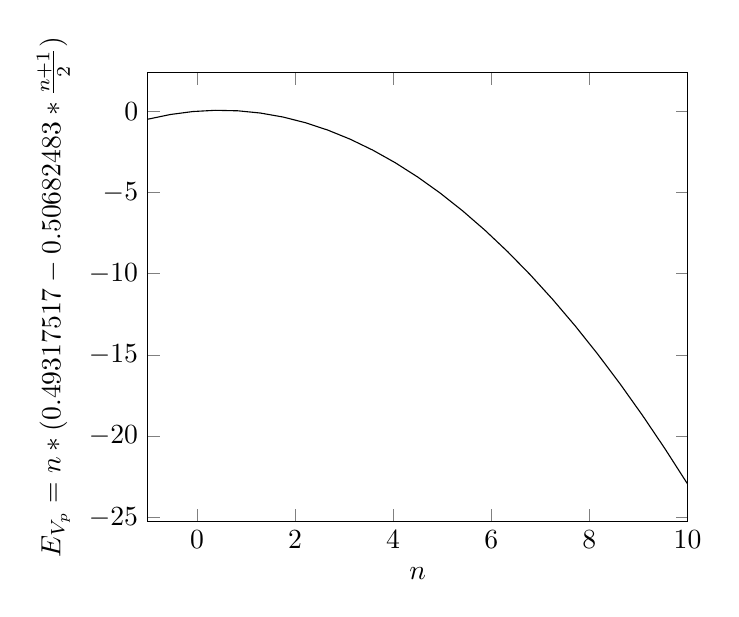
\begin{tikzpicture}
  \begin{axis}[ 
  	xmin=-1,
  	xmax=10,
    xlabel=$n$,
    ylabel={$E_{V_p}=n*(0.49317517-0.50682483*\frac{n+1}{2})$}
  ] 
    \addplot [domain=-1:10]{x*(0.49317517-0.50682483*((x+1)/2))}; 
  \end{axis}
\end{tikzpicture}
\end{center}
from (5.6), For betting \emph{BANKER BOX} our $r=0.95$ and $p_l=p_p$ we have:
\begin{center}
$E_{V_b}=n(r(1-p_l)-p_l\frac{n+1}{2})$\\
$E_{V_b}=n(0.95*(1-0.49371517)-\frac{n+1}{2}*0.49371517)$\\
$E_{V_b}=n*(0.95*(0.50682483)-0.49371517\frac{n+1}{2})$\\
(5.8) \\
\end{center}
\begin{center}
\begin{tikzpicture}
  \begin{axis}[ 
  	xmin=-1,
  	xmax=10,
    xlabel=$n$,
    ylabel={$E_{V_b}=n*(0.95*(0.50682483)-0.49371517\frac{n+1}{2})$}
  ] 
    \addplot [domain=-1:10]{x*((0.95*0.50682483)-0.49371517*((x+1)/2))}; 
  \end{axis}
\end{tikzpicture}
\end{center}
From these equations, we can see that all EVs are negatives when $n\geq1$ when $n=1$ then it is the same as \emph{Flat Bet}. \\

\subsubsection{Add Half, Reduce Half}
I did not have a name for this strategy.  It is somewhat a variation of the martingale's but in \emph{half}.  How does it work?  \\

For every lost hand, we will \emph{add} half of the previous bet to be the next bet.  And we will \emph{reduce} half the previous bet every time we win (not start at the minimum bet.  for $a_n$ is bet amount at $n$ hands we have:
\begin{center}
$a_n= a_{n-1}+(a_{n-1}*\frac{1}{2})$\\
$a_n= a_{n-1}*\frac{3}{2}$\\
\end{center}

We should round up for any not-integer results.  So that if we started with $1$ we will have a series of bet size raising as $1, 2, 3, 5, 8, 12, 18, 27, ...$ as we can see this reduced the number we increase in the series comparing to Martingale's: $1,2,4,8,16,32,64,...$ \\

When the last hand wins, we reduce half of the previous bet. That is, at $a_n$, the bet amount is:\par
\begin{center}
$a_n=a_{n+1}-(a_{n+1}*\frac{1}{2})$\\
$a_n=a_{n+1}*\frac{1}{2}$\\
$a_n=\frac{a_{n+1}}{2}$\\
\end{center}

as before we should round-up for any not-integer results.  and for that all bets are according to the previous bet amount then we will have no winning series but some of them are shown below:\\
\begin{tabbing}
\hspace*{5px}\=41:\hspace*{5px} \=21,\hspace*{5px} \=11,\hspace*{5px}\=6,\hspace*{5px} \=3,\hspace*{5px}\=2,\hspace*{5px}\=1\\
\hspace*{5px}\=62:\hspace*{5px} \=31,\hspace*{5px} \=16,\hspace*{5px}\=8,\hspace*{5px}\=4,\hspace*{5px}\=2,\hspace*{5px}\=1\\
\hspace*{5px}\=93:\hspace*{5px} \=47,\hspace*{5px} \=24,\hspace*{5px}\=12,\hspace*{5px}\=6,\hspace*{5px}\=3,\hspace*{5px}\=2,\hspace*{5px}\=1\\
\hspace*{5px}\=27:\hspace*{5px} \=14,\hspace*{5px} \=7,\hspace*{5px} \=4,\hspace*{5px}\=2,\hspace*{5px}\=1\\
\hspace*{5px}\=18:\hspace*{5px} \=9,\hspace*{5px} \=5,\hspace*{5px} \=3,\hspace*{5px} \=2,\hspace*{5px}\=1\\
\end{tabbing}

\begin{center}
\emph{\textbf{*note*}} \\
\end{center}

Because of that defensive strategies are betting a larger amount after the previous losses.  all the defensive betting strategies are all fallen into one of the \emph{Gambler Fallacies} that says \emph{"It is more likely you will win the next round if you lose the in the previous round"} which is \textbf{false}. 

\subsubsection{Fibonacci}

There is a sequence of numbers called Fibonacci numbers.  This is a very famous sequence since it is believed to be seen all over nature.\\
\\
This is how the sequence goes.\\

$1, 1, 2, 3, 5, 8, 13, 21, 42, 63, 105, ...$\\

From the above sequence we have a sequence of Fibonacci numbers in an equation shown below:\par
\begin{center}
 $a_n=a_{n-1}+a_{n-2}$.  \\
\end{center}

To use this sequence is for every loss, we move our bet for a larger amount one position.  For each win, we move back to the lower amount \textbf{two} positions\\

\subsubsection{Labouchere}
For this strategy, sometimes it is called "Split Martingale" it is because of how it is managing the betting amount.\\

For this strategy, you must pick a target and divide it into several bets using your minimal bet.  For example, to get a 1,000\$ if your minimum bet is 100\$ then you will have 10 bets of 100\$.  write it down in a series. Every bet you bet the sum amount of the left end and the right end of the series.  For this example, your first bet will be 200\$.  For every loss, you write down the amount to the right side of the series. The next bet will be 100\$ plus newly write down 200\$, this next bet will be 300\$. After each win, you scratch out these numbers on both ends and continue as before with the number that is still listed.\\

\subsubsection{Defensive Betting Systems in Summary}
\emph{Defensive Betting Systems} mostly keep players in the winning zone but with risking a large bankroll to back up the strategies.  To me, it feels greater, at least for a longer time than \emph{Aggressive Betting Systems}.  But remember, if you keep betting, it will eventually be a long streak and the winnings will be returned to the casinos (hopefully this happened after some winnings).  But if the long losing streak is at the beginning of the session, this large loss is very hard to accept by most people.\\  

The nature of this type of strategy guarantees winning if you have an infinite bankroll or no betting limits.

\subsection{Aggressive Betting Systems}

Most of the time, they are called \textbf{Positive Betting Systems}, but I'd call it an \emph{Aggressive} betting system, and they don't give out positive EVs.  These are betting system that would normally have the same properties and increments and the reducing system as the Defensive Betting Systems but in reverse.  \\

Aggressive Betting Systems will increase the bets when the previous winning rounds.  In other words, your bet will grow as the winning goes, so that sometimes these types of strategies are called \emph{flowing with the trends} strategies.  and be mostly used in the Stock Market.\\

\subsubsection{Oscar's Grind}
Add one unit that you win, but do not vary your bet either lose or tie hands.\\

\subsubsection{Paroli}
Play minimal at 1 unit bet and add one unit when you win, until you have three wins in a row, then go back to 1 unit bet.  For each loss, go back to one unit.\\

\subsubsection{Aggressive Betting Systems in summary}
To me, this type of strategy is not my favorite.  And trust me, the math is just the same as the defensive betting systems with the same increasing and decreasing bet strategy. This type of strategy has a good nature of using luck.  Its nature is to use a small bankroll to win big, with luck.  But trust me, most of the time, it does not feel good playing with this type of strategy, since players will be in the losing zone longer than the winning zone, and hope for a large win.

\subsection{Informative Betting Systems}
Good news! until now there is only this type of Betting System that gives out a positive EV.  The bad news is, it is hard to implement and does not guarantee that you will win on every session.  Until now, the only informative betting around is \emph{Card Counting} which is not very easy to implement on the table.  Players have put their minds into every game, and every card dealt to gather information from the situation on the table as much as possible, to gather all information on the table and calculate count risk and chance, also the right amount should bet on each hand.  This is sure will make the game even more boring and not fun to play.  Moreover, the casinos know about this, so they try to prevent \emph{card counters} in all sorts of ways.\\

If you want to learn more about counting cards for Baccarat, or Blackjack you can search for books online, but I am sure it will not very profitable.  And remember no strategy is guaranteed to win in the short run.  Even though, in the long run, you win money, but there will be some bad luck day, or days, repeatedly.  You will have to have good bankroll management and very discipline to be able to profitably implement it on the table.\\

\subsection{Betting systems in summary}

To summarized information on Progressive Betting Systems, I can just say that most of them do not work in the long run.  They are fun and can make you feel excited playing, or implement these strategies.    \\

So far, there is only one type of betting system that works.  That is informative betting systems.  At this moment there is only one strategy found, \emph{Card Counting}.\\

From math and tests, in theories, any betting systems that are not the informative betting system type, or cannot mathematically prove their EV to be positive, are not working in the long run.  So, don't buy them. \\

\clearpage
\section{Other Games}
After explored Baccarat and found that there is no way you can win in Baccarat.  I learned some other games like \emph{Blackjack}, \emph{Roulette}, \emph{Poker}, \emph{Tiger Dragon}.\\

\subsection{Tiger Dragon}
Tiger Dragon is something like a quick version of the Baccarat.  With the same two choices, you can make a \emph{Tiger} Box or a \emph{Dragon} Box.  each box will be dealt with one card and the start to compare the point.  The lowest score of the game is Ace count as 1 point. J as 11, Q as 12, and K as 13 points. \\

The payout of the game is 1:1 but for a tie, it will not be a push.  you will have to pay $\frac{1}{2}$ for the bet.  Let see all the outcomes to calculate the probability.  For this, we can calculate the Probability as:\\

\begin{table}[htb]
\centering
\begin{tabular}{|c|c|c|c|}
\hline
card & Win cases & Lose cases & Tie Cases\\
\hline
A:&	0&		12&	1\\
2:&	1&		11&	1\\
3:&	2&		10&	1\\
4:&	3&		9&		1\\
5:&	4&		8&		l\\
6:&	5&		7&		1\\
7:&	6&		6&		1\\
8:&	7&		5&		1\\
9:&	8&		4&		1\\
10:&9&		3&		1\\
J:&	10&	2&		1\\
Q:&	11&	1&		1\\
K:&	12&	0&		1\\
\hline
\end{tabular}
\caption{Above table shows the outcomes of the game Tiger Dragon}
\end{table}

from the table above we can see that we have 78 Win Cases 78 Loose Cases and 13 Tie.  On either box Tiger or Dragon, it is 78 winning cases.  that is $\approx\frac{78}{169}=0.461538462\approx46.154\%$ winning probability and 91 winning cases.  that is $\approx\frac{91}{169}=0.538461538\approx53.846\%$ losing probability.  These two cases are different in payout, one is -1, and one is -$\frac{1}{2}$.  \\

\subsubsection{Calculating EV}

To calculate EV for Tiger and Dragon we must calculate it separately.  Let $E_V$ is Expected Value of the Tiger Dragon, $p_w$, $p_l$, $p_t$ are winning, losing, and tie probabilities accordingly we can write EV equation as below:\\ \\
From equation (4.1) we have:
\begin{center}
$$EV=\sum_{i=1}^{c_w}E_{R_i}+\sum_{i=1}^{c_l}E_{L_i}$$\\
$EV=p_w - p_l - \frac{1}{2}p_t$ \\
$EV=0.461538462 - 0.461538462 - \frac{1}{2}0.076923077$ \\
$EV=- \frac{1}{2}0.076923077$\\
$EV=-0.038461538$\\
\end{center}

As we can see EV for Tiger Dragon game has $EV=-0.038461538$ equally on both sides that is you will lose \approx3.846\% of your bet every time you bet.\\

\subsection{Roulette}
Roulette is a big table with a spinning wheel with 36 numbers on the table.  Because 36 is a very good number because it is the least common number of multiple numbers, players can bet on any number any dozen, odds, or even numbers. These are \textbf{Betting Options} for roulette:\par
\begin{description}
\item[Individual] Players are allowed to bet on any individual (including 0 and 00 in American Roulette) number and the payout is 35:1
\item[Odd/Even] Players are allowed to bet on these \emph{almost} half-half bets by choosing any bet on \textbf{odd} numbers, or \textbf{even} numbers, the payout is 1:1
\item[Red/Black] These 50/50-type bets are just about the same.  Players can  choose any bet on \textbf{Reds}, or \textbf{Black} numbers, the payout is 1:1
\item[High/Low] another \emph{almost} half-half bets that players can choose.  The players can bet on \textbf{High} numbers (19 and above), or \textbf{Low} numbers (18 and below), the payout is also 1:1.
\item[Dozen/Column] These are 12 number bets locate either on the bottom or on the side of the table, the payout is 2:1
\item[Line] These are 6 number sets Locate on the side of the table, the payout is 5:1
\item[Corner] Also known as square or Box of Four bets, this allows players to bet 4 number at the same time, the payout is 8:1.
\item[Street] I a way that you can bet across 3 columns in line, that allows players to bet 3 number set.  The payout is 11:1.

\end{description}

To calculate EV for Roulette it is important to know that they are two types of Roulette table.  The wheel with 00 \emph{Double Zero} and 0 is called \textbf{"American Roulette"}, another one has only one 0 on the table that is called \textbf{"European Roulette"}. 

\subsubsection{European Roulette}
Now we know that European Roulette has only 36 numbers to bet in those red/black, odd/even, high/low, ... and so on areas, but it has a total of \textbf{37} numbers in the wheel including the \emph{GREAN ZERO}.  now let us do the calculation\\
\\
The EVs for each bet option we have for European Roulette.  Let $E_{V_i}$, $E_{V_b}$, $E_{V_d}$, $E_{V_l}$, $E_{V_c}$, $E_{V_s}$ as Expect Values for Individual, Binary, Dozen, Line, Corner, Street:\\
\\
\textbf{Individual Numbers Bets}
\begin{center}
$E_{V_i}=35 * \frac{1}{37} - 1 * \frac{36}{37}$\\
$E_{V_i}=35*0.027027027 - 0.972972973$\\
$E_{V_i}=-0.027027027$\\
\end{center}   
\textbf{Binary Bets}
\begin{center}
$E_{V_b}=\frac{18}{37} - 1 * \frac{19}{37}$\\
$E_{V_b}=0.486486486 - 0.513513514$\\
$E_{V_b}=-0.027027027$\\
\end{center} 
\textbf{Street Bets}
\begin{center}
$E_{V_s}=11 * \frac{3}{37} - 1 * \frac{34}{37}$\\
$E_{V_s}=11*0.081081081 - 0.918918919$\\
$E_{V_s}=-0.027027027$\\
\end{center}  
\textbf{Corner Bets}
\begin{center}
$E_{V_c}=8 * \frac{4}{37} - 1 * \frac{33}{37}$\\
$E_{V_c}=8*0.108108108 - 0.891891892$\\
$E_{V_c}=-0.027027027$\\
\end{center}  
\textbf{Line Bets}
\begin{center}
$E_{V_l}=5 * \frac{6}{37} - 1 * \frac{31}{37}$\\
$E_{V_l}=5*0.162162162 - 0.837837838$\\
$E_{V_l}=-0.027027027$\\
\end{center}  
\textbf{Dozen Bets}
\begin{center}
$E_{V_d}=2 * \frac{1}{37} - 1 * \frac{36}{37}$\\
$E_{V_d}=2*0.324324324 - 0.675675676$\\
$E_{V_d}=-0.027027027$\\
\end{center}  

As we can see, all bet areas can be calculated for the same EV value.  which is -0.027027027\approx-2.7\%, that is when you play European Roulette you will lose money by 2.7\% of your bet by average.

\subsubsection{American Roulette}
In the same way, we calculate European Roulette, we can calculate EV for all betting options using the same method.  But American Roulette has a total number of \textbf{38} not 37 like European Roulette, therefore we can write out the EV solutions as following:\\
\\
\textbf{Individual Numbers Bets}
\begin{center}
$E_{V_i}=35 * \frac{1}{38} - 1 * \frac{36}{38}$\\
$E_{V_i}=35*0.026315789 - 0.973684211$\\
$E_{V_i}=-0.052631579$\\
\end{center}   
\textbf{Binary Bets}
\begin{center}
$E_{V_b}=\frac{18}{38} - 1 * \frac{20}{38}$\\
$E_{V_b}=0.473684211 - 0.526315789$\\
$E_{V_b}=-0.052631579$\\
\end{center} 
\textbf{Street Bets}
\begin{center}
$E_{V_s}=11 * \frac{3}{38} - 1 * \frac{35}{38}$\\
$E_{V_s}=11*0.078947368 -0.921052632$\\
$E_{V_s}=-0.052631579$\\
\end{center}  
\textbf{Corner Bets}
\begin{center}
$E_{V_c}=8 * \frac{4}{38} - 1 * \frac{34}{38}$\\
$E_{V_c}=8*0.105263158 - 0.894736842$\\
$E_{V_c}=-0.052631579$\\
\end{center} 
\textbf{Five Number Bets}
\begin{center}
$E_{V_f}=6 * \frac{5}{38} - 1 * \frac{33}{38}$\\
$E_{V_f}=6*0.131578947 - 0.868421053$\\
$E_{V_f}=-0.078947368$\\
\end{center}  
\textbf{Line Bets}
\begin{center}
$E_{V_l}=5 * \frac{6}{38} - 1 * \frac{32}{38}$\\
$E_{V_l}=5*0.157894737-0.842105263$\\
$E_{V_l}=-0.052631579$\\
\end{center}  
\textbf{Dozen Bets}
\begin{center}
$E_{V_d}=2 * \frac{12}{37} - 1 * \frac{26}{38}$\\
$E_{V_d}=2*0.315789474 - 0.684210526$\\
$E_{V_d}=-0.052631579$\\
\end{center}  

Same as European Roulette all bet options are giving the same EV, besides Five Number Bets which only available in American Roulette (we represent it EV using $E_{V_f}$).  That only payout 6:1 and EV of -0.078947368\approx-7.89\%.  For all other betting options, we have an EV of -0.052631579\approx-5.26\%, That is when playing American Roulette players will lose their money by an average of \approx5.26\% of their bet amount.\\

In summary, Roulette either American or European Roulette all gives the negative EV.  That is, they are not a good investment, so \textbf{do not} play them.  But if you choose to have fun and sure that you can afford this entertainment, make sure you choose European Roulette for a better EV and save money.\\
  

\subsection{Poker}
\paragraph{ }Poker is a kind of game that players do not play against the casino.  But  to make money out of the commission of the game, the casino takes a commission from the pot, very much like the cost of renting their properties.  The rate that the casino takes from the pot varies from place to place but generally about 2.5-10\% of the pot amount. \\

Taking commission out of the pot, makes poker become a \emph{negative-sum game} which means that if you divided the money from the pot back to each player, it will be lesser than it was put in.  That means, in total, it already has a negative EV.  For this pot, the player will have to use luck, strategy, skill to acquire it, which makes poker, a game of skill.\\

Poker is also one-of-a-kind games that required skill and some talent is needed.  There are strategies in poker that use against other players.  A skilled player can almost guarantee to win and make money from the game so that we have professional poker players.\\

There are many types of poker, the very famous one is called \textbf{Texas Hold'em} It is so famous that, is ESPN (a world well-known sports channel) puts this game into their game of interest and broadcast it worldwide!\\

I do not know much about poker in detail, and I know, I will never make a good poker player.  Although, I still believe the EV is still playing a big part in this game. But let us not go too deep. on this one.

\subsection{Blackjack}
Blackjack is sometimes called \textbf{21} because this 21 number plays a major part in this game.  In this game, all players are playing against the dealer.  

The rule is after players are dealt 2 cards and the dealer 1 face-up card, at this time the game already has begun, and they are situations:\\
\begin{description}
\item[blackjack] if a hand (either a player's or the dealer) has a point of 21 with 2 cards 10s and Aces, this is called \emph{Blackjack}.  As long as the dealer doesn't also have a Blackjack the player will be paid 1.5:1.  If the dealer has a blackjack, all players that do not have blackjack will lose their bet instantly.
\end{description}

Before I describe the rule any further, I should explain some terms of the game.\\

\begin{description}
\item[Busted] if a hand (either a player's or the dealer) has a point over 21, that hand considers losses, and the bet is collected right away.  Since the dealer performs last, if the dealer also a bust, the bet will not be returned, not considered a push, and all remaining players will be paid the winning amount.
\end{description}

At this moment players can take action either \emph{hit}, \emph{stand}, \emph{double}, \emph{split}, or \emph{surrender}.\\

\begin{description}

\item[Stand] means the player does not want any more cards or does not take any further action.
\item[Hit] the player can acquire one more card as many times as he likes, until he \emph{stands}, or is \emph{busted}.
\item[Double down] in case of only two cards, some casinos allow this action.  It is that the player can double their bet amount and receive only one more card, and automatically stand for the hand.
\item[Split] in case of only two cards with the same value, some casinos allow splitting hands up to a certain number of hands.  The player must add the same bet amount to split his/her hand to another hand.  Then the hand will be spitted into two same initial value cards.  
\item[Surrender] some casinos offer this option, most of the time only allowed for initial action.  For this choice, the dealer will collect half of the bet and the hand is over. 
\end{description}

After all, the players are done taking actions, all \emph{stand}, the dealer will check his/her cards and will have to hit until his/her points more than 16.  In this case, the dealer can be either 17-21 or \emph{bust}.  Then we compare the score in the players' hand and the dealer's, the one closer to 21 but not over 21 wins!  If the scores are equal, that is called \emph{pushes} the bets are returned to the players in full 1:1 amount.\\

From the above action choices, players can take any action according to their situations and information.  So that they are some strategies that are used on the tables.  Some of them are:
\begin{description}
\item[Mimic the Dealer] Since they can see the dealer has their rules, they assume that this is for the casino's best interest, then they should do it too. This will raise the house edge to 5.48\%.
\item[Assume ten in the hole] Player assumes that the next card is a ten. This is one of the worst strategies in Blackjack, it raises the house edge to 10.03\%.
\item[Never Bust] Some detail are almost the same as the above strategy but for this strategy, they will just try not to bust themselves and always try to stay in the game to the end.  Assume that they play the correct basic strategy, they will stand on all hard total of 12 or above. This strategy raises the house edge to 3.91\%.
\item[Basic Strategy] Is a mathematically calculated optimum strategy for each dealer up card, and the player score.  Let us discuss it in detail, now.
\end{description}

\subsubsection{Basic Strategy}
In this sub-section, I will show the table of basic strategy, of a certain rule.  I could not help you remember all the actions in all cases.  But I assure you, it is possible to remember it all, with practice and training.\\

Below is a basic strategy assume that they play with \infty decks of cards, dealer stands on soft 17, double down available on any two cards, Ace split once, and double after split is allowed, and blackjack pays 3 to 2.\\

\clearpage
\begin{table}[htb]
\centering
\textbf{Dealer's Up Cards}\\
\begin{tabular}{|c|c|c|c|c|c|c|c|c|c|c|}

\hline
\textbf{Hard Hand} & A & 2 & 3 & 4 & 5 & 6 & 7 & 8 & 9 & 10 \\
\hline
5-8 & H & H & H & H & H & H & H & H & H & H\\
9  & H & H & D & D & D & D & H & H & H & H\\
10 & H & D & D & D & D & D & D & D & D & H\\
11 & H & D & D & D & D & D & D & D & D & D\\
12 & H & H & H & S & S & S & H & H & H & H\\
13 & H & S & S & S & S & S & H & H & H & H\\
14 & H & S & S & S & S & S & H & H & H & H\\
15 & H & S & S & S & S & S & H & H & H & R\\
16 & H & S & S & S & S & S & H & H & R & R\\
17+& S & S & S & S & S & S & S & S & S & S\\
\hline
\textbf{Soft Hand} & A & 2 & 3 & 4 & 5 & 6 & 7 & 8 & 9 & 10 \\
\hline
13 & H & H & H & H & D & D & H & H & H & H\\
14 & H & H & H & D & D & D & H & H & H & H\\
15 & H & H & D & D & D & D & H & H & H & H\\
16 & H & H & D & D & D & D & H & H & H & H\\
17 & H & H & D & D & D & D & H & H & H & H\\
18 & H & S & D & D & D & D & S & S & H & H\\
19+& S & S & S & S & S & S & S & S & S & S\\
\hline
\textbf{Split Hand} & A & 2 & 3 & 4 & 5 & 6 & 7 & 8 & 9 & 10 \\
\hline
A & P & P & P & P & P & P & P & P & P & P\\
2 & H & H & H & P & P & P & P & H & H & H\\
3 & H & H & D & P & P & P & P & H & H & H\\
4 & H & H & H & H & H & H & H & H & H & H\\
5 & H & D & D & D & D & D & D & D & D & H\\
6 & H & H & P & P & P & P & P & H & H & H\\
7 & H & P & P & P & P & P & P & H & H & H\\
8 & P & P & P & P & P & P & P & P & P & P\\
9 & H & P & P & P & P & P & S & P & P & H\\
10& S & S & S & S & S & S & S & S & S & S\\
\hline

\end{tabular}
\caption{Shows Blackjack Basic Strategy}
\end{table}

But for those who in an emergency, need to use it fast, there is a simplified version of this, although it is not as good, but close enough.  Remember these 9 rules\\
\\
\textbf{Hard Hands}
\begin{itemize}
\item Always stand on 17 or more.
\item For Dealer has 7 or more, the player with a score of 12 to 16: always hit.
\item Always double down on 10 or 11 if the dealer has a lower value card.
\item Below than 10: hit
\end{itemize}
\textbf{Soft Hands}
\begin{itemize}
\item Always Hit for 17 or less
\item Always stand on 18 or more.
\end{itemize}
\textbf{Split Hands}
\begin{itemize}
\item Never Split 10s, 5s.
\item Always Split As, and 8s.
\end{itemize}
If the above situations are not the case...\\
\\
\textbf{General Hands}
\begin{itemize}
\item Always Stand when the dealer shows 2 to 6
\end{itemize}

\subsubsection{calculating EV}

To calculate this game's EV, it is not as simple as Baccarat, Tiger Dragon, or Roulette.  Because it involves many actions and decisions which depending on the situation and previous action the player takes.  But all and all, for a certain strategy it is calculatable.  \emph{Michael Shackleford} AKA \emph{Wizard of Odds} has a calculated EV for blackjack basic strategy on his website.  and on his Youtube channel; he even has video clips show how he calculated the optimal strategy and the EV of the strategy.  It is pretty much of finding all the possibilities of cases, and EV of each case and then sum them all up.\\
\\
If you are interested
\begin{itemize}
\item \url{https://wizardofodds.com/games/blackjack/}
\item Blackjack Basic Strategy for Infinite Decks\\ \url{https://www.youtube.com/watch?v=wJsGnXgrGvg}
\item Blackjack house edge with infinite decks\\ \url{https://www.youtube.com/watch?v=jCF-Btu5ZCk}
\end{itemize}

The calculated basic strategy EV from \emph{Wizard of odds} is -0.00485\approx0.485\% that is in the long-run player can expect to lose money about 0.5\% of his/her bet amount on average.

\subsection{Gambling outside of Casino}
In life, even when we know or do not know recognize it or not chance and risk are involved in our lives all our lifetime.  If you do not trust me ask those who do gambling for business.  
\subsubsection{Gambling for business}
You might ask me, is there gambling for business?  Yes, there is.  Trust me when I say people in this business industry know best about life's uncertainties.\\

The life insurance business companies, they know that risk involves in our everyday life.  When we wake up, take shower, travel, when we cook, even when we sleep, the risk is always upon us all.  uncertainty is their business, our lives are their game of gambling and business.\\ \\
\textbf{Life Insurance}\\
They will invest or gamble in the knowledge of the chance male and female health risk, and lifespan is the risks and chances.  Consider the insurance premium we paid, to the insurance company is their returns, the insurance policy we would benefit money is their losses.  From these factors, they can calculate EVs, and how much they should charge their customers, how much they should pay for each customer.  \\

For example, let us say, on average they are 6.8 death out of 1000 people in the year 2015, that the death rate of \approx.0068 or \approx0.68\% per year.  if the insurance company willing to pay 200,000\$ per case that is $E_L\approx200,000 * 0.0068\approx1360\$$ that is the amount they had to pay each customer on average.  That is for the business to survive, the premium that the company will collect from customers must be higher than this amount.  Which probably would also include profit, management cost, and safe margins\\

As you know for males and females of different ages, their health risks and lifespan are  different.  That is why the insurance premiums are differed by age and gender, or even country.  \\

\subsubsection{Lottery}
This is a big legal way of gambling.  It has all the same property of a risk-reward system built into it.  It is designed to have a big profit for the government that funds it.  And we can even calculate EV for the lottery.  \\

Let suppose a lotto costs 10\$ and they are sold 1,000,000 pieces across the country.  if the reward for the winner is 2 million dollars, that means the government still has 8 million dollars left as a profit. Let us write it down using math, we have:\\
\\
\textbf{for the government side} let $c$ is the cost of each lotto, $p$ is pieces sold, for the chance they acquire the money is 100\%=1, $r$ is the reward payout, if the government is good and promised to payout every time then they will have a risk of $k$ = 1 = 100%:
\begin{center}
$E_V= c*p*1 - r * k$\\
$E_V= 10 * 1,000,000 - 2,000,0000 $\\
$E_V= 8,000,000$\
\end{center}


That is if the government arranges lotto like this, every time they will have 8,000,000\$ in profit.  The government might spend another million more to spend on creating small prices to give lotto buyers higher hope, and still have 7,000,000\$ left as profit.\\
\\
\textbf{for the buyer, side} let $p$ is a price of each lotto for the chance they spend the money is 100\%=1, $r$ is the reward payout by the government, with a chance $c=\frac{1}{1,000,000}$:

\begin{center}
$E_V= r * c - 10$\\
$E_V= 2,000,000*\frac{1}{1,000,000} - 10 $\\
$E_V= -8$\\
\end{center}

Consequently, if the government took another million to make them 500 more small prizes, then the total $E_V$ are improved to $E_V=-7$ but it still is a negative number.\\

we can see that for each buyer it is a negative Expected Value, but I know it might be fun to take a chance to win big money with just 10\$, right?

\subsubsection{Stock Market}

Stock Market, Forex, and Crypto Currencies Market are very much alike, but in most countries, the stock market is legal, others not. Stock Market is one other place you can gamble.  You can buy a stock and hope the price rise and sell it later when the price is high.  But that is not always the case. \\

The nature of the stock market is a \emph{zero-sum game}, that is the amount of money the buyer buys stocks and the money sold to the seller is equal and balance.  But in real life, there is a third party who added a fee to the price when every we buy and sell stocks that make the stock market no longer a \emph{zero-sum game}.  That is there will be someone (in this case: the brokers) that will always benefit and make a profit from all actions.  This is the same as playing poker in a casino, and the casino takes out some commission from the pot.\\

Since the game in the stock market is no longer a \emph{zero-sum game}, this indicates that if the asset in the market is divided equally among players it will not have the same value as they put in.  This is dangerous for all the players, so in other words, it has a total negative EV.  Now, this also depends on the strategy of the investors which we will not discuss in this paper.\\

\clearpage
\section{Gambler Fallacies}

\subsection{Luck}
One thing I sometimes ask myself and I have been asked a lot in the gambling world is "does luck has anything to do with gambling?"  As an engineer, I will always believe in the math we got.  However, luck does play out on each small session we play or invest in.  That is some 100 games we win, some 100 games we lose, some 100 games we win big, some 100 games we lose big!  I will not argue with those who believe in those supernatural things.  So, do whatever you believe, this time you might win, this time you might lose.  All this is to just  point out, in the end, math will play out as we calculated.\par

\subsection{Supernatural}
Sometimes things very much less likely to happen, happened.  This happens a lot in the field of gambling, one in thousands, in millions, or in billions also happens. so, \textbf{get used to it}.  You must look at everything as it has the same probability to happen as other cases. \\

For example, if let you shuffle a deck of card, believe it or not, you have just made a miracle.  You have just made something extraordinary out of that deck of cards. For every time you shuffle a deck of cards, it is almost guaranteed that there has never been a deck of cards arranged in this combination (permutation) before! Why? Because all possible permutations of a deck of cards are $C_1^{52}=52!$ That is $\approx8.065817517094388 * 10^{67}$ (8 follow with 67 zeroes).  What you just did (shuffling the deck of card) that was epic no one of a kind since the beginning of the universe!  It is 1 out of $\approx8.065817517094388 * 10^{67}$, and that all happen by your power, not by any supernatural power.\\

One other example, in August 2020, a lotto winner was the number 999997 that does not look so natural right?  It very much looked as if it was made up, or there was someone behind it.  But it is not.  Just remember the number 999997 has the same probability $\frac{1}{1,000,000}$ same as 125987, or 789546, or any other number with 6 digits. When 785412 can occur, but why 999997 would be considered unnatural.  Because that is how human is biased, we were born with this instinct.  We all tend to find an explanation, of things, and when we do not know-how, some of us turn to ignorance and believe including the supernatural.\\

The occurring of these few chance event, always it brings us the question, was anything behind all this. Or even make us think this must be a work of something we cannot see.  \\\

This led people to believe in supernatural phenomenons. as I said, in the previous topic, so \emph{do whatever you believe}.  It does not matter this time you win or lose, but in the long run, the result will be as mathematical predicted.\\

\subsection{Due to Win}
There are some beliefs in the world of gambling.  Most of the gamblers would think that if in this gameplay he loses then the next gameplay he is more likely to win.   That is false.  That is not the case.  if the average game probability is 50-50, and this gameplay you lose, it does not mean that the next game win probability will be 75\%.  (As I told you, I too fell into this trap) The next game probability is still 50-50. \\

Unless you know the combination of the cards left in the shoe and able to calculate it fast enough, every game in Baccarat, Blackjack is about the same average probability.  And that is the beginning of \emph{card counting} as mentioned in \emph{Informative Betting Strategy}\\

\subsection{Near Miss}
This is not a belief, not an idea, not anything just an excuse for the gamblers to gamble more.  It just does not base on anything, not science, nor math but it all based on emotion, intention to gamble more, and gamble again.\\

What this is, for example, a player was playing European Roulette, and he bet on number 9.  But after the wheel spun, the outcome was 8.  That is a "near miss" scenario.  This is false, there is no science that after 8 next will be 9 nor 7.  The probability is still the same $\frac{1}{37}$ for every spin.  But the gambler will just feel they are close to win, nearly win that round.\\

Although I said this does not base on any science it affects on psychology level after this happens.  After the gambler sees a near-miss scenario, the reward system still does affect the gambler the same way as he already won.  And that will control his behavior to play continuously. \\



\clearpage
\section{The Gambling Morale and Society}
\subsection{Investing and Gambling}
Investing and Gambling are involve around asset, money, chance, risk, return, loss.  So, in terms of the component, it the same thing.  But there are differences between the two.  \\
\subsubsection{The Concepts}
Think of the students in a classroom at a final exam.  This involves choices, scores, and information. Those who learn, study hard, will always have a better grade, than those who do not study and finish their final exam with guesswork.\\

Investing and gambling are the same as the students in the above example.  They are all taking exams, but with a different context, they are different in action, and mindset.  Investing is more like those who study and gather all the information they can before an exam, while gambling is more like the student who takes the exam not knowing anything and hope for the best.\\

That is when we say investing and gambling are the same thing, that is not far from the truth.  It depends on the act of investors.  If the learned  study and make an educated investment that is called investment, but if they just interesting in a chance and invest in it without any study, that is gambling.\\

In the stock market, FOREX, cryptocurrencies all have both investors and gamblers, so in the long run, the gamblers will always lose their money.  Investors who study and take all the information they have into account before making a decision will profit in the long run.\\


\subsubsection{What Separate Investors and Gamblers}
From what I learned in the gambling and investing world I found it astounding that these two groups of people are very alike in some way but there is only a thin line dividing separate them.  Those are:\par
\begin{description}
\item[knowledge:] This topic can be considered as the main fact that differentiates them.  While investors will make their decisions based on knowledge, reasons but gamblers will make their decisions by guessing, liking, and believing.
\item[Choice:]  From the knowledge those investors acquired, some gamblers can almost consider as investors if they make their choice wisely.  If one knew the EV of such investment is a negative number and still invest in that investment, that is an act of gambling.  They can say do it for fun or hope to win big in the short run, but it is guaranteed to lose money in the long run.
\item[Disciplines:] Since those investors have their knowledge and aim for high profit and lower their risks, therefore, they will have their own set of rules, and actions.  While the gamblers will just do, act, invest as they please.
\item[Risk Management:] One of the investors' disciplines would be how they manage their risk and investments.   The investors will not risk their money they do not have AKA invest in borrowed money unless they have calculated EV that is way more profitable than the interest rate, or no interest tie to the debt.  The gamblers are likely to borrow, sell their assets just to gamble! 
\item[Final Results:] In the long run the smart investors will be profitable, but gamblers will undoubtedly lose all their money in the long run.
\end{description}

\subsection{Cheating}
Cheaters exist everywhere and can all be suspected.  Since the casinos already have higher mathematical advantages they do not need to cheat.  I did not mean that they do not cheat or will not cheat.  that is why those countries with legal casinos will have a government department dedicate to inspect them in all aspects.\\

On other hand, the casinos are very suspicious of all their players, that any of them might be a cheater.  Since the casino is to make money.  They do not afford to lose any of their income to the cheaters.  That is why we see cameras at every corner on the casino floors, they have guards to guard all the entrances and the \emph{cages} (This is how the casino call their \emph{Cashiers}).  They inspect every move of the player, every gameplay, and every behavior. \\

Nowadays, people are still trying to cheat the casino, trying to win the casino.  Even they advertise that you can \emph{win big}, they do not like you to win big!  They like you to \emph{win sometime}, that you will come back and play again.  So, if you win big, that is ok, but if you consistently win, that will surely bring up a red flag to the casino to check you out.\\
\subsubsection{Land-Based Casinos}
From the theory of EV, the odds, and the house edge built-in to all the games, the casino is almost guaranteed to be profitable.  A land-based casino is built everywhere, legally, or illegally.  For the countries those land-based casinos are legal, they are inspected and closely observed to check their methods and management.  \\
\begin{description}
\item[Legal Land-Based Casinos:] For the reason above the legal land-based casino is less likely to be a scam, fraud, or cheat on the players.  
\item[Illegal Land-Based Casinos:] On the other hand, illegal land-based casinos in those countries that gambling is not legalized, casinos are not closely observed or inspected that open opportunity for the land-based casino to physically cheat trick, or mafia their players.  Since they can open casinos illegally, it is most likely that they are do not worry about the law.  Even all the games have a house edge built-in to the game itself, but greed is the power that pushes people to do things.  Some not so standardized games can be seen in this type of casinos.  for the reasons explained about the illegal land-based casinos, it is not as safe as a legal land-based casino.  For they do not afraid of the law, anything could happen in the casinos, so, it can be considered dangerous being in one. 
\end{description}

For the reasons above, if gambling is what you do, I encourage you to go to only legally open casinos, if losing money is not what you worry about, but at least be sure only go to legal one for your safety.\\

\subsubsection{Online Casinos}
Do not think they are the same, bun an online version, I must warn you. This is different from a land-based casino.  An online casino is everywhere, legally, and illegally.  They are types of games provided on online casino websites. digital games, and live dealer games.  I will not touch on the digital part, since we all know that the digitalized games, can do anything smelly.  And anyone who played it virtually has accepted that risk.  So let us focus on the live dealer games.  But to understand this business, you will have to know how the system works for online casinos. \\
\begin{description}
\item[The Software Providers] This refers to businesses that provide service to casino platforms to use their gaming services that the platform does not have to manage their own online casino licensing and management. This is where the live dealers are broadcast, and digital software is provided.\\

Most of the time the software provider has no intention to cheat for they do not gain from cheating the gambler, they gain from payment from the platform.  And the software will be regularly checked by the country of their origins to be fair and legal.  There might be some errors or bugs in the system but those are not considered cheating.  They can also cheat but they might stay in the business for long.\\

\item[The Casino]  This part will refer to the business part, the man who open an online casino, doing all account management, market it, decorating the website, earning licenses, payment management, and providing customer support.\\

The casino refers to those who run the business, they hold the money, and pay the money.  Some digital game settings are set by the platform, house edge, and payout, etc.  They are mostly be considered cheaters and fraud.  Since they can use some strategy to hold back the money in their pocket as long as they can, or even worst! not paying you.  So, be careful!\\
\end{description}

I'm not saying that they are no genuine online casinos, but since it is online and remote play there is not much you can do about any error or their spooky actions.  Or if you are in a country that gambling is illegal, that is the worst-case scenario, that no one can help you about it, if things go sideways.\\


\subsection{Gambling Addiction}
So far, we do not have any positive EV bet in a casino.  That means, there is no true winning, in the long run.  Winning it, in the long run, is just a fantasy.  So, one last thing I need to talk about before ending this paper is \emph{Gambling Addiction}.\\

Gambling Addiction is simply the worst of all addictions.  It is worse than those who addict to drugs, sport, cigarettes, or alcohol.  The addicts are stimulated in many ways chemically, biologically, environmentally, ethically which makes them deeply addicted and harder to quit.\\

Researchers found that gambler tends to have high stress which stimulates the brain to give out happiness hormones, there are 3 types of these addictive hormones, that make gambling harder to quit than other types of addicts.  \\
\begin{description}
\item[Endorphin] is released when the body or mind is under stress, in pain but it is also an addictive substance that the human body can produce.    
\item[Dopamine] will be released when a person or animal is rewarded, to support a certain action to be repeated.  This hormone is released a lot in children.  That one part of how we learn and study while we are young.
\item[Serotonin] is a happy hormone released when you think of a past experienced moment which will support their feeling of wanting to do that or be in that moment again. 
\end{description}

As we can see that while gambling, gamblers unconsciously trained themselves to be addicted to the help of Dopamine, at that moment they are stressed, then we have a happy moment from the effectiveness of the Endorphin hormone. And when we are away from gambling, anything related to that moment such as smells, scenes will bring up the memory of the gambling.  Which makes them want to go back and gamble again!\\

Other than harder to quit, but it is also more dangerous than other types of addicts.  The other type of addicts might have health issues, not strong enough by the effect of the drugs, but gambling is different.  The addicts will have their full-body strength as normal people, their mind quick as normal, but they want to gamble!  They want it bad that they can do anything to gamble. \\

They might hurt someone, might rob, might sell their body parts, might sell their assets, or even their family just to gamble!\\
\begin{center}
\textbf{I hope you are not one of them!}
\end{center}

\subsection{Professional Rules}
As suggested in the beginning, this paper is not to promote gambling or vise versa but just to give out knowledge. Players can make up their minds whether or not to gamble.  But in this sub-section, I just want to give some suggestions, in case you'll gamble anyway.  They are rules that professional gamblers always follow, or players are guaranteed to be doomed. 

\begin{description}
\item[Do not play a game you do not understand] it is already a bad idea gambling but it is worst if you play the game you do not know or understand the rules.  Rules of the games, game of life, physically, financially, mentally, mathematically.
\item[Do not play with the money you do not have] if you do not have money to play, do not play.  Do not lend, or borrow money to play.  Do not use your credit card to gamble, do not sell your assets to gamble.  Remember if you gamble, you are guaranteed to lose in the long-run, with bad luck might be a short-run.  So, just play only that you can afford, and remember to think of the loss as a form of entertainment fees, \textbf{"Do not chase losses"}.
\item[Play smart:] since you are guaranteed to lose in the long-run.  It is best to select a game with the lowest house edge.  and bet on specific low house edge bets.  This will help you save lots of money, and with the casinos' comps might even out your losses.  If we look at the losses as entertainment fees, this as well lowers the entertainment fees. 
\item[Be conscious at all times:] In the casino, there will be all sorts of distractions.  You'll have to be sure that you are conscious all the time to keep and implement the three rules at all times.  Never play for profit, never try to get back what was lost.  Most of all, if there is no mathematically proven winning strategy, do not think of gambling professionally or think of it as an investment.  Keep in mind, \textbf{"Gambling is not an investment"}.
\end{description}















\clearpage
\section{Summary}
\paragraph{ }From what I described, we learned, we know that there is no game in the casino, online or offline, that has a positive EV.  Some game is worse than others, at the same time some strategies are also worse than others.  So, do not bother buying any progressive betting system from the internet, none of them works. \\

Some informative systems are cool and proven mathematically, but it is not found to be  very profitable, needed hard work, and not fun to play or implement, so why bother.  It is better to go find a job anyway.\\

I am not saying do not gamble, there are reasons people still gambling and the casinos are still standing until this day.  There are still some gamblers that can balance their lives and having fun at the same time.  Others might just earn enough money just to gamble.  Some have their own set of rules to gamble and earn money not having fun at all. Some gamble with their lives risks their social, assets, family.  These are the gamblers' mindsets.  So, choose which kind of life you pick as a gambler, an investor, or an addict.\\

Finally, I encourage all players to learn math, trust in math, and implement them in your life.  Take your action rationally, be careful, do not careless, and stay conscious.  Your action might define you, but you control your action!
































  


\clearpage
\begin{thebibliography}{9}
 
\bibitem{r1} 
Wizard of Odds
\\\texttt{\url{https://www.wizardofodds.com}}

\bibitem{r2}
\hypertarget{2}{}
Wikipedia: Life Insurance
\\\texttt{\url{https://en.wikipedia.org/wiki/Life_insurance}}


\bibitem{r3}
Mortality Table
\\\texttt{\url{https://www.irs.gov/pub/irs-drop/n-19-26.pdf}}

\end{thebibliography}
\end{document}
